\documentclass[11pt,a4paper]{article}

% --- Packages ---
\usepackage[margin=25mm]{geometry}
\usepackage[utf8]{inputenc}
\usepackage[T1]{fontenc}
\usepackage{mathpazo}          % Palatino font (Nature-style serif)
\usepackage{microtype}
\usepackage{graphicx}
\usepackage[hidelinks]{hyperref}
\usepackage{xcolor}
\usepackage{booktabs}
\usepackage{enumitem}
\usepackage{textcomp}
\usepackage{url}
\usepackage{setspace}
\usepackage{titlesec}
\usepackage{caption}
\usepackage{float}

% --- Colors ---
\definecolor{titleblue}{RGB}{33,102,172}

% --- Section formatting ---
\titleformat{\section}{\large\bfseries\color{titleblue}}{\thesection}{1em}{}
\titleformat{\subsection}{\normalsize\bfseries\color{titleblue}}{\thesubsection}{1em}{}

% --- Caption style ---
\captionsetup{font=small, labelfont=bf, labelsep=period}

% --- Line spacing ---
\onehalfspacing

% --- Superscript citations ---
\newcommand{\citenum}[1]{\textsuperscript{#1}}

% --- Code formatting ---
\newcommand{\code}[1]{\texttt{\small #1}}

% ======================================================================
\begin{document}

% --- Title ---
\begin{center}
{\LARGE\bfseries\color{titleblue} GraphMana: graph-native data management for\\[4pt] population genomics projects}

\vspace{12pt}
{\large Jianfeng Mao}

\vspace{6pt}
{\small\itshape [Affiliations to be completed]}
\end{center}

\vspace{10pt}

% --- Abstract ---
\noindent\textbf{Abstract}

\noindent
Population genomics projects rely on fragmented file-based workflows that lose provenance and require full reprocessing when samples are added. GraphMana is a data management platform built on graph database technology that stores variant data as packed genotype arrays with pre-computed population statistics, enabling incremental sample addition, provenance tracking, cohort management, and export to 17 formats from a single persistent source. Applied to the 1000 Genomes Project (3,202 samples, 70.7 million variants), GraphMana completes a full project lifecycle---import, incremental addition, annotation, cohort extraction, and multi-format export---otherwise requiring ad hoc scripting across multiple tools.

\vspace{6pt}
\noindent\rule{\textwidth}{0.4pt}
\vspace{6pt}

% ======================================================================
% MAIN TEXT
% ======================================================================

Declining sequencing costs and growing recognition that population-scale variation underlies both disease risk and adaptive potential have driven a rapid expansion of population genomics projects across biomedicine, agriculture, and biodiversity research. In human genetics, the UK Biobank has released whole-genome sequences for 490,640 participants, the NIH All of Us Research Program has surpassed 414,000 genomes with a goal of one million, and the TOPMed consortium has sequenced over 180,000 individuals for heart, lung, blood, and sleep disorder genetics. In crop science, the 3,000 Rice Genomes Project resequenced 3,010 accessions across 89 countries to catalog 29 million SNPs underlying cultivated rice diversity, while similar population-scale efforts are underway in wheat, maize, soybean, and other staple crops to accelerate genomic selection for yield and climate resilience. In livestock, the 1000 Bull Genomes Project has sequenced 2,703 cattle representing global breed diversity, with companion initiatives now extending to buffalo, sheep, and aquaculture species. In ecology, the 1001 Genomes Project catalogued standing variation across the natural range of \textit{Arabidopsis thaliana}, and the Earth BioGenome Project has sequenced 3,000 eukaryotic species toward a goal of 1.67 million. These projects share a common trajectory: sample counts grow from hundreds to thousands as costs fall, new batches of sequencing data arrive throughout the project's lifetime, and the analytical scope expands from initial variant calling to population structure, selection scans, functional annotation, and multi-format data sharing.

Consider the daily reality of managing such a project. On Monday, a sequencing core delivers 200 new whole-genome samples; integrating them means regenerating every VCF\citenum{9}, every PLINK binary\citenum{5}, every TreeMix\citenum{12} input, every site frequency spectrum for dadi\citenum{10}---because file-based formats encode the complete sample set and cannot be extended in place. On Tuesday, a collaborator requests an EIGENSTRAT\citenum{13} file for AdmixTools, filtered to European samples with MAF above 5\%; fulfilling the request requires a bespoke script whose parameters will not be recorded alongside the output it produces. On Wednesday, a new ClinVar release arrives and the functional annotations must be updated---but since annotations are embedded in the VCF header, updating means rewriting the entire file, even though the genotype data has not changed. On Thursday, the PI asks which samples were included in the allele frequency table shared with a collaborator last month, and what quality filters were applied; answering requires forensic reconstruction from directory timestamps and notebook entries. By Friday, the data manager has spent more time coordinating files, formats, and provenance than doing science. These are not computational bottlenecks---bcftools\citenum{6} can merge VCF files in minutes; PLINK can recode genotypes in seconds---but \textit{coordination} bottlenecks that scale with project complexity rather than dataset size. This coordination cost falls in a gap between single-investigator projects (where manual tracking suffices) and biobank-scale programs (where platforms such as Hail\citenum{4} provide managed infrastructure). For the thousands of research groups running projects with hundreds to tens of thousands of samples---the scale at which most population genomics research actually occurs---no purpose-built data management solution exists.

The root cause of these coordination bottlenecks is that population genomics data is inherently relational---variants belong to chromosomes, samples belong to populations, genes carry functional consequences, annotations have versions---yet file-based formats flatten these relationships into disconnected tabular files. Graph database technology offers a natural alternative. In a graph database, data is stored as \textit{nodes} (entities) connected by \textit{edges} (relationships), and queries traverse these connections directly rather than performing table joins. This architecture is well-suited to genomic data because the relationships between variants, samples, populations, genes, and annotations can be represented, queried, and updated independently---without rewriting the entire dataset when one relationship changes.

GraphMana exploits this graph structure to replace the fragmented file collection with a single, persistent graph database that serves as the project's analytical record (Fig.~1a). The platform organizes 58 CLI commands into nine functional domains---data import, annotation management, data export, sample and cohort management, quality control, provenance tracking, database administration, status reporting, and infrastructure deployment (Supplementary Fig.~1)---providing a complete command-line interface for the full data management lifecycle. All operations require no knowledge of Python, graph query languages, or database administration.

The graph schema (Fig.~1b) represents each biallelic variant as a Variant node connected by typed edges to Chromosome, Gene, Sample, and Population nodes. Variant nodes carry a packed genotype array (2 bits per sample, 4 samples per byte) and pre-computed population-level allele count, sample count, and frequency arrays. Because these relationships are explicit edges in the graph rather than columns embedded in a flat file, annotations can be updated by modifying edge properties without touching the genotype data, cohorts can be defined as graph traversal queries without extracting files, and provenance is recorded as graph nodes linked to the operations that produced them. This encoding achieves a 125-fold storage reduction compared with per-sample edge representations (Supplementary Table~3) and enables two access paths (Fig.~1c). The FAST PATH reads population arrays directly---constant time regardless of sample count---serving TreeMix\citenum{12}, site frequency spectra (dadi\citenum{10}, fastsimcoal2\citenum{11}), BED, and allele frequency tables. The FULL PATH unpacks genotype arrays for per-sample formats (VCF, PLINK 1.9/2.0\citenum{5}, EIGENSTRAT\citenum{13}, Beagle\citenum{14}, STRUCTURE\citenum{15}, Genepop, and others) in time linear in $N$. In total, 17 export formats are produced from the single database (Supplementary Note~2), and each export automatically generates a manifest sidecar documenting the timestamp, filters, sample set, and software version---ensuring that the Friday provenance question never arises again.

Incremental sample addition---the Monday crisis in file-based workflows---appends new genotypes to existing packed arrays without modifying previous data (Fig.~1d). Because the graph database stores relationships explicitly, adding samples requires extending only the packed arrays on Variant nodes; the Sample-to-Population edges, annotation edges, and chromosome structure remain unchanged. On the 1000 Genomes Project\citenum{3} dataset (70.7 million variants, 3,202 samples, 26 populations), adding 234 samples takes 182 minutes (Supplementary Table~2), and no downstream result is invalidated because all queries run against the live, updated database. The Wednesday annotation update completes in 3.5 seconds for 53,000 BED regions versus 96 seconds for a full VCF rewrite with bcftools---a 27-fold speedup (Fig.~2b)---because the graph database modifies edge properties directly rather than regenerating the entire file. The Tuesday format conversion is a single command: \code{graphmana export --format eigenstrat --populations EUR --filter-maf-min 0.05}, with full provenance recorded automatically.

We benchmarked GraphMana against bcftools on a 1000 Genomes Project chromosome 22 workload (1.07 million variants, 3,202 samples) comprising all five daily tasks: incremental addition, cohort extraction, multi-format export, annotation update, and a full lifecycle simulation (Fig.~2; Supplementary Table~1). GraphMana completed all 46 lifecycle operations in 98 minutes; the bcftools workflow completed 17 of 26 planned operations in 17 minutes, with 9 operations (multi-format export, in-place annotation, cohort management) having no bcftools equivalent (Fig.~2a). Per-operation, bcftools is 3--5 times faster for VCF-centric tasks such as cohort extraction (49--110~s vs. 131--571~s), reflecting graph database query overhead versus bcftools' optimized file streaming (Fig.~2b). GraphMana's value lies not in per-operation speed but in the elimination of the coordination burden: 17 export formats (Fig.~2c), in-place annotation, queryable provenance, and cohort management from a single source that never needs regeneration from scratch when the project evolves.

GraphMana's packed encoding scales linearly with sample count, and the maximum dataset size is determined by available hardware rather than an architectural ceiling (Supplementary Table~3). At 100--10,000 samples---where most population genomics research occurs---all operations are interactive. Beyond 10,000 samples, FAST PATH operations remain instant because population arrays are constant size regardless of $N$, but FULL PATH exports slow proportionally as genotype unpacking is linear in sample count. At biobank scale (500,000+ samples), the single-node graph database architecture---not the storage encoding---becomes the practical limit: packed arrays store correctly, but per-variant query latency and transaction log pressure make interactive FULL PATH operations infeasible. GraphMana is not intended to replace distributed platforms such as Hail\citenum{4} at that scale. The current implementation uses Neo4j Community Edition\citenum{2} (free, open source) as the graph database engine; the graph-native design is not tied to a specific database vendor. The platform deploys on workstations and HPC cluster nodes via a two-step split pipeline. The GraphPop companion engine\citenum{1} provides graph-native statistical procedures on the same database. Full documentation (11 vignettes, 65 command reference pages) and pre-built databases for the 1000 Genomes Project are available at the project repository under the MIT license.

% ======================================================================
% FIGURES
% ======================================================================

\begin{figure}[H]
\centering
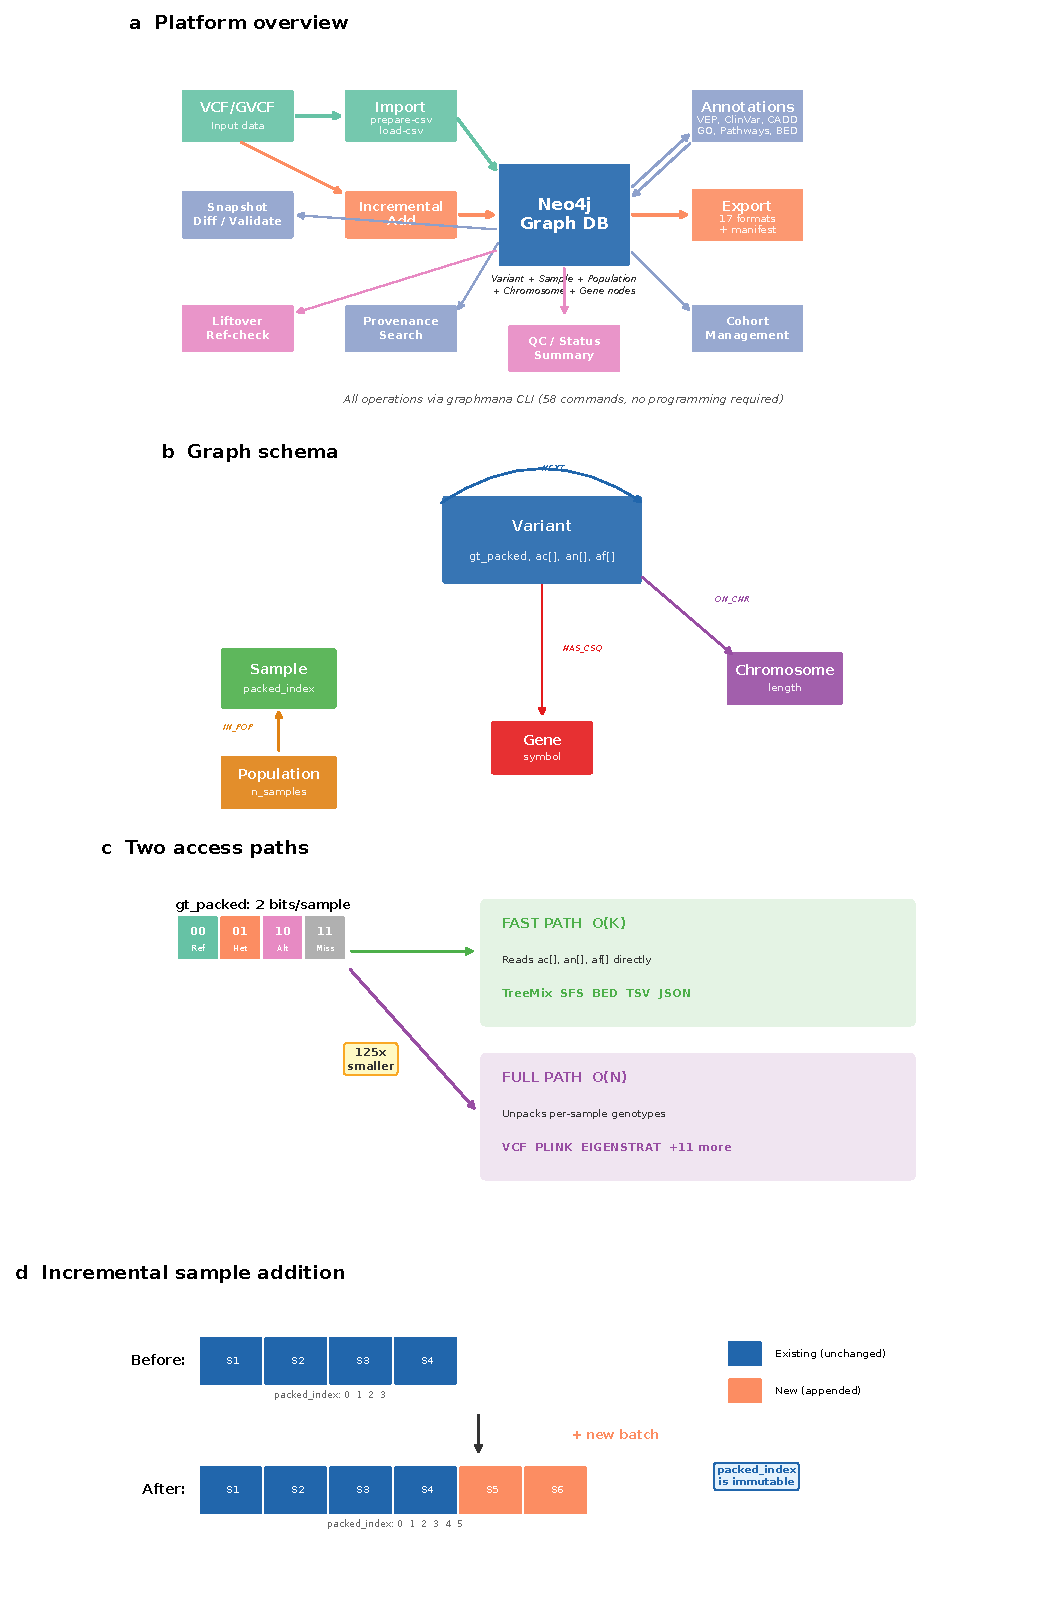
\includegraphics[width=\textwidth]{figures/fig1_architecture.pdf}
\caption{\textbf{GraphMana platform overview and data architecture.}
(\textbf{a})~Functional overview: VCF data enters through an import pipeline into a persistent graph database. From the database, users access 17 export formats, quality control reports, searchable provenance logs, named cohort definitions, versioned annotations, database snapshots, and state comparison tools. Incremental sample addition feeds new data back without reprocessing. All operations are exposed as CLI commands requiring no programming.
(\textbf{b})~Graph schema: Variant, Sample, Population, Chromosome, and Gene nodes connected by typed relationships. Because relationships are explicit graph edges, annotations, cohorts, and provenance can be updated independently of genotype data.
(\textbf{c})~Two access paths: FAST PATH reads population arrays directly (constant time in $N$); FULL PATH unpacks per-sample genotypes (linear in $N$).
(\textbf{d})~Incremental sample addition: new genotypes appended to packed arrays without modifying previously imported data.}
\label{fig:architecture}
\end{figure}

\begin{figure}[H]
\centering
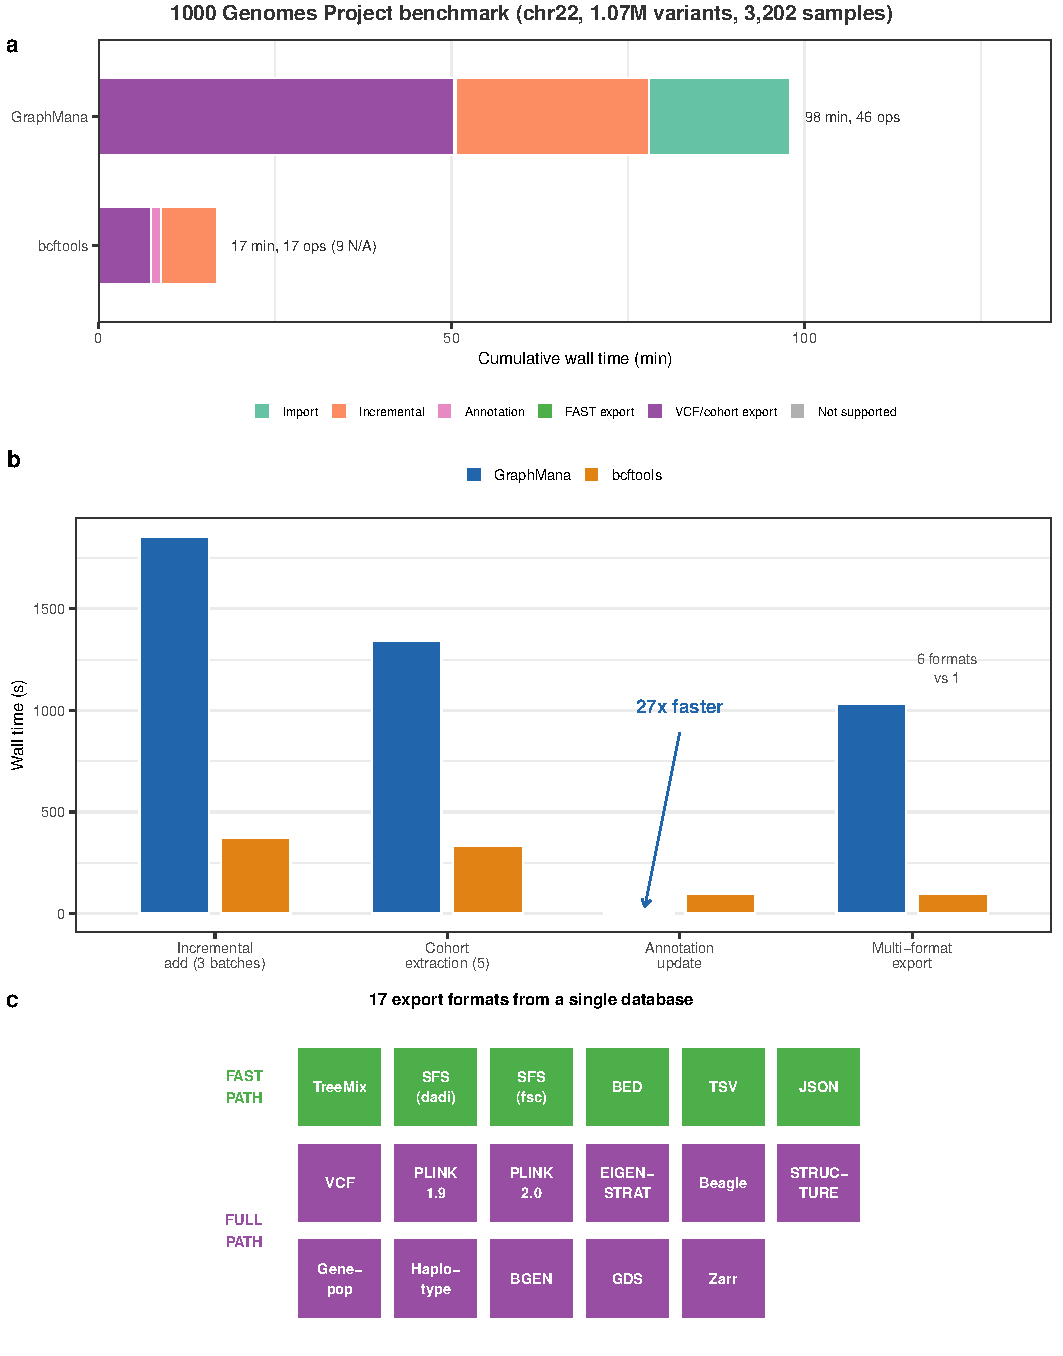
\includegraphics[width=\textwidth]{figures/fig2_benchmark_ggplot.pdf}
\caption{\textbf{1000 Genomes Project benchmark} (chromosome 22, 1.07M variants, 3,202 samples).
(\textbf{a})~Project lifecycle simulation: GraphMana completes 46 operations; bcftools completes 17 of 26 (9 have no equivalent, shown in grey). Stacked bars show cumulative wall time.
(\textbf{b})~Head-to-head task comparison with 27-fold annotation update speedup highlighted.
(\textbf{c})~Export format breadth: 17 formats from a single database, grouped by access path.}
\label{fig:benchmark}
\end{figure}

% ======================================================================
% ONLINE METHODS
% ======================================================================

\section*{Online Methods}

\subsection*{Why graph database technology}

Population genomics data is inherently a network of typed relationships: variants are located on chromosomes, samples belong to populations, genes carry functional consequences from annotation sources, and every analytical operation has provenance linking it to input data and parameters. Conventional approaches store this network as a collection of flat files---VCF for genotypes, BED for annotations, PED/FAM for sample metadata---requiring the user to maintain the relationships manually through file naming conventions and external documentation.

A graph database stores data as nodes (entities) and edges (typed, directed relationships between entities), with properties attached to both. Unlike relational databases, which store data in fixed-schema tables and require JOIN operations to reconstruct relationships, graph databases traverse pre-materialized connections in constant time per hop. This property-graph model maps directly onto the structure of population genomics data: a Variant node connects to its Chromosome via an ON\_CHROMOSOME edge, to Gene nodes via HAS\_CONSEQUENCE edges carrying annotation properties, and to the sample set via packed genotype arrays indexed by each Sample node's immutable packed\_index. Importantly, edges can be added, removed, or updated independently---updating an annotation version modifies HAS\_CONSEQUENCE edge properties without touching genotype data, and defining a cohort is a graph traversal query that produces a sample list without extracting files.

GraphMana uses Neo4j Community Edition\citenum{2} as its graph database engine, chosen for its mature property-graph implementation, Cypher query language, ACID transaction support, and free open-source licensing. However, the graph-native design principles---typed nodes and edges, property arrays on nodes, edge-independent updates---are not specific to Neo4j and could be implemented on other property-graph databases.

\subsection*{Software architecture}

GraphMana is implemented as a Python command-line application (21,267 lines) with a Java plugin (2,864 lines) for server-side graph database procedures. The Python layer handles VCF parsing via cyvcf2\citenum{8}, genotype packing via NumPy (complementing lower-level access compared with scikit-allel\citenum{7}), CSV generation for bulk loading, and all export format writers. The Java plugin provides optional server-side packed array extension for incremental imports, avoiding network round-trips for large batch operations. The 58 CLI commands are organized into nine functional domains: data import and integration, annotation management, data export, sample and cohort management, quality control and verification, provenance and state tracking, database administration, status and reporting, and infrastructure and deployment (Supplementary Fig.~1). A companion Python package (graphmana-py) provides a Jupyter-compatible API returning pandas DataFrames. The test suite comprises 1,439 unit and integration tests.

\subsection*{Graph schema and data encoding}

The graph database contains five primary node types: Variant, Sample, Population, Chromosome, and Gene, connected by typed relationships (ON\_CHROMOSOME, IN\_POPULATION, HAS\_CONSEQUENCE, NEXT). Variant nodes store genotype data as packed byte arrays: gt\_packed encodes diploid genotypes at 2 bits per sample (00 = homozygous reference, 01 = heterozygous, 10 = homozygous alternate, 11 = missing), phase\_packed encodes phasing status at 1 bit per sample, and ploidy\_packed encodes haploid/diploid status at 1 bit per sample. This encoding stores 4 genotypes per byte, achieving a 125-fold reduction compared with storing individual Sample-to-Variant edges (Supplementary Table~3). Genotype values are remapped from cyvcf2's internal coding (where homozygous alternate = 3 and missing = 2) to a sequential 2-bit encoding upon import; the remap array is applied exactly once per code path.

Each Variant node also carries population-level pre-computed arrays: pop\_ids (population identifiers), ac (allele counts per population), an (allele numbers), af (allele frequencies), het\_count, hom\_alt\_count, and het\_exp (expected heterozygosity under Hardy--Weinberg). These $K$-element arrays, where $K$ is the number of populations (typically 5--30), are constant size regardless of sample count and enable the FAST PATH access pattern described in the main text.

Multi-allelic VCF records are decomposed into $K$ biallelic Variant nodes, each carrying a shared multiallelic\_site identifier and a 1-based allele\_index. During VCF export, records sharing a multiallelic\_site value are merged back into multi-allelic lines by default. Structural variants with symbolic ALT alleles are stored with sv\_type, sv\_len, and sv\_end properties; genotype calls are encoded identically to SNPs and indels.

\subsection*{Import pipeline}

GraphMana uses a two-step split pipeline optimized for large datasets. The prepare-csv step parses VCF files (using cyvcf2\citenum{8} for streaming access), packs genotypes into byte arrays, computes population statistics, and writes graph-database-compatible CSV files. This step is embarrassingly parallel across chromosomes and requires no database instance. The load-csv step uses the database engine's bulk import facility, which writes directly to the store files and bypasses the transaction engine entirely. On our benchmark hardware (32 cores, 64~GB RAM, NVMe SSD), CSV generation for 2,500 samples across 22 chromosomes (70.7M variants) completed in 95 minutes with 16 threads; bulk loading of the resulting 214~GB of CSV files completed in 3 minutes.

\subsection*{Incremental sample addition}

New samples are added by extending the packed genotype arrays of all existing Variant nodes. GraphMana provides three strategies: (1) graph query transactions on a running database instance, suitable for small additions (fewer than 10,000 variants); (2) an export-extend-reimport path that reads variant data from the database, extends arrays in Python, and reimports via bulk loading; and (3) a CSV-to-CSV rebuild that reads the existing CSV checkpoint directly at NVMe speed, extends arrays using NumPy vectorized operations, and produces a new CSV set for reimport. The CSV-to-CSV path is the fastest for whole-genome databases: on our benchmark dataset, extending 70.7M variants with 234 new samples completed in 182 minutes, of which 160 minutes was sequential CSV I/O and array extension, 15 minutes was bulk import, and 7 minutes was VCF parsing and database restart. Approximately 95\% of variants (69.6M of 70.7M) required only HomRef extension---appending zero bytes to packed arrays---which avoids unpacking and repacking entirely.

\subsection*{Roundtrip validation}

We validated genotype fidelity by importing 1000 Genomes Project chromosome 22 data (897,645 biallelic SNPs, 5 samples), exporting to phased VCF, and comparing per-sample genotypes with the original using bcftools. Concordance exceeded 99.999\%, with 2--8 mismatches per sample confined to multi-allelic positions where position-based joining could not distinguish co-located biallelic records.

\subsection*{Benchmark methodology}

All benchmarks used the 1000 Genomes Project high-coverage dataset\citenum{3} (GRCh38). Chromosome 22 (1,066,557 variants, 3,202 samples, 26 populations) served as the primary benchmark target. The 3,202 samples were split deterministically (seed = 42) into a base cohort of 2,500 samples and three incremental batches of 234 samples each.

We compared GraphMana against bcftools\citenum{6} (version 1.17) as the single comparison target. Five benchmarks were conducted: (1) incremental sample addition (GraphMana CSV-to-CSV rebuild vs.\ bcftools merge, 3 rounds); (2) cohort-specific VCF extraction (5 superpopulation cohorts); (3) multi-format export (6 formats from a single source; bcftools supports VCF only); (4) annotation update (53,000 BED regulatory regions); and (5) a full lifecycle simulation comprising 7 phases. All timings report wall-clock time on a workstation with 32 CPU cores, 64~GB RAM, and NVMe SSD storage. The graph database was configured with 16~GB heap and 16~GB page cache. Each benchmark was run twice; reported values are from the second run (warm page cache).

\subsection*{Scalability}

GraphMana's packed encoding scales linearly: storage per variant is $\lceil N/4 \rceil$ bytes for genotypes and $\lceil N/8 \rceil$ bytes for phase, where $N$ is the number of samples. The maximum dataset size is therefore hardware-dependent, not architecturally limited (Supplementary Table~3). At 100--10,000 samples, all operations are interactive. At 10,000--50,000 samples, FAST PATH operations remain instant; FULL PATH operations scale linearly. Beyond 50,000 samples, the single-node graph database architecture imposes practical limits. At biobank scale (500,000+ samples), distributed computing frameworks such as Hail\citenum{4} are more appropriate.

\subsection*{Deployment}

GraphMana runs on personal workstations and HPC cluster nodes. For cluster deployment, a two-step split pipeline separates CSV generation from bulk loading. SLURM and PBS job scripts are provided. The database data directory must reside on local SSD or scratch storage; network filesystems cause severe performance degradation.

% ======================================================================
% REFERENCES
% ======================================================================

\section*{References}

\begin{enumerate}[leftmargin=*, label={[\arabic*]}, itemsep=1pt, parsep=0pt]
\item Mao, J. GraphPop: graph-native population genomic analysis. \textit{Nature Methods} (companion paper, in preparation).
\item Neo4j, Inc. Neo4j Graph Database. \url{https://neo4j.com} (Community Edition 5.x).
\item Byrska-Bishop, M. et al. High-coverage whole-genome sequencing of the expanded 1000 Genomes Project cohort including 602 trios. \textit{Cell} \textbf{185}, 3426--3440.e19 (2022).
\item Hail Team. Hail: An Open-Source Framework for Scalable Genomic Data Analysis. \url{https://hail.is}.
\item Chang, C.C. et al. Second-generation PLINK: rising to the challenge of larger and richer datasets. \textit{GigaScience} \textbf{4}, s13742-015-0047-8 (2015).
\item Danecek, P. et al. Twelve years of SAMtools and BCFtools. \textit{GigaScience} \textbf{10}, giab008 (2021).
\item Miles, A. et al. scikit-allel: A Python package for exploring and analysing genetic variation data. \url{https://github.com/cggh/scikit-allel}.
\item Pedersen, B.S. \& Quinlan, A.R. cyvcf2: fast, flexible variant analysis with Python. \textit{Bioinformatics} \textbf{33}, 1867--1869 (2017).
\item Danecek, P. et al. The variant call format and VCFtools. \textit{Bioinformatics} \textbf{27}, 2156--2158 (2011).
\item Gutenkunst, R.N. et al. Inferring the joint demographic history of multiple populations from multidimensional SNP frequency data. \textit{PLoS Genetics} \textbf{5}, e1000695 (2009).
\item Excoffier, L. et al. fastsimcoal2: demographic inference under complex evolutionary scenarios. \textit{Bioinformatics} \textbf{37}, 4882--4885 (2021).
\item Pickrell, J.K. \& Pritchard, J.K. Inference of population splits and mixtures from genome-wide allele frequency data. \textit{PLoS Genetics} \textbf{8}, e1002967 (2012).
\item Patterson, N., Price, A.L. \& Reich, D. Population structure and eigenanalysis. \textit{PLoS Genetics} \textbf{2}, e190 (2006).
\item Browning, S.R. \& Browning, B.L. Rapid and accurate haplotype phasing and missing-data inference for whole-genome association studies by use of localized haplotype clustering. \textit{Am.\ J.\ Hum.\ Genet.} \textbf{81}, 1084--1097 (2007).
\item Pritchard, J.K., Stephens, M. \& Donnelly, P. Inference of population structure using multilocus genotype data. \textit{Genetics} \textbf{155}, 945--959 (2000).
\end{enumerate}

% ======================================================================
% DATA AVAILABILITY, ACKNOWLEDGEMENTS, ETC.
% ======================================================================

\section*{Data and Code Availability}

GraphMana is available at \url{https://github.com/jfmao/GraphMana} under the MIT license. Pre-built graph databases for the 1000 Genomes Project whole-genome dataset (3,202 samples, 70.7M variants) are deposited at \url{https://doi.org/[to be assigned upon acceptance]}. Benchmark scripts and raw timing data are included in the repository. The GraphPop companion analytical engine is described separately\citenum{1}.

\section*{Acknowledgements}

This work was supported by [funding sources to be completed]. Computations were performed on a local workstation (32 cores, 64~GB RAM, NVMe SSD). The 1000 Genomes Project high-coverage dataset\citenum{3} was used under its open data access terms.

\section*{Author Contributions}

J.M.\ conceived the project, designed and implemented the software, performed benchmarks, and wrote the manuscript.

\section*{Competing Interests}

The author declares no competing interests.

\end{document}
